\documentclass[11pt]{article}

\usepackage{a4wide}
\usepackage{amsmath,amssymb}
\usepackage[english]{babel}
\usepackage{enumitem}
\usepackage{float}
\usepackage[bottom]{footmisc}
\usepackage{graphicx}
\usepackage[utf8]{inputenc}
\usepackage{listings}
\usepackage{multicol}
\usepackage{tikz}

%========== DEFINITIONS & MACROS ==========%

\definecolor{comment}{rgb}		{0.38, 0.62, 0.38}
\definecolor{keyword}{rgb}		{0.10, 0.10, 0.81}
\definecolor{identifier}{rgb}	{0.00, 0.00, 0.00}
\definecolor{string}{rgb}		{0.50, 0.50, 0.50}

\newcommand{\figref}[1]{see figure~\ref{#1}}
\newcommand{\secref}[1]{see section \ref{#1} on page \pageref{#1}}
\newcommand{\appref}[1]{see appendix \ref{#1} on page \pageref{#1}}
\newcommand{\txtref}[2][]{see {\it #1} \ref{#2} on page \pageref{#2}}
\newcommand{\code}[1]{{\tt #1}}
\newcommand{\file}[1]{{\tt #1}}
\newcommand{\imp}{\rightarrow}
\newcommand{\norm}[1]{\lVert#1\rVert}
\newcommand{\unit}[1]{\frac{#1}{\norm{#1}}}
\newcommand{\mat}[1]{\text{\bf #1}}
\newcommand{\transpose}[1]{1^{\text{T}}}

\newcommand{\codefig}[5]
{
\begin{figure}[H]
    \lstinputlisting[firstnumber=#3,firstline=#3,lastline=#4]{../../src/#2}
    \caption{Code excerpt #5 (#2)}
    \label{code:#1}
\end{figure}
}

\setdescription{leftmargin=\parindent, labelindent=\parindent}

\lstset
{
    language=C++,
	% general settings
	numbers=left,
	frame=single,
	basicstyle=\footnotesize\ttfamily,
	tabsize=2,
	breaklines=true,
	% syntax highlighting
	commentstyle=\color{comment},
	keywordstyle=\color{keyword},
	identifierstyle=\color{identifier},
	stringstyle=\color{string},
}


\title
{
    {\Large Individual Assignment 6} \\
    Introduction to Computer Graphics
}

\author
{
    Casper B. Hansen \\
    University of Copenhagen \\
    Department of Computer Science \\
    {\tt fvx507@alumni.ku.dk}
}

\date{last revision \today}

\begin{document}

\clearpage\maketitle\vspace{1in}
\begin{multicols}{2}
    \begin{abstract}
        We discuss the concept of parametric surfaces, taking particular
        interest in Bezier patch surfaces and general surfaces.
        
        The reader is expected to have read the previous assignment, in which
        many mathematical definitions used are presented, but it not required
        to have any prior knowledge of the material presented, which builds
        onto to that. Some parts require knowledge of partial differential
        equations and derivatives. For the code the reader is expected to
        have some basic understanding of linear algebra and the C++ language.
    \end{abstract}
    \vfill\columnbreak\tableofcontents\vfill
\end{multicols}
\thispagestyle{empty}\newpage

\section{Theory}

\subsection{Parametric Surfaces}
A parametric surface $Q$ is --- in 3-dimensional space --- defined on
$\mathbb{R}^2 \imp \mathbb{R}^3$, taking a vector argument $(s,t)$ for which
$Q(s,t_0)$, where $t_0$ is a fixed value, is a parametric curve along $s$, and
vice versa for $Q(s_0,t)$, where $s_0$ is a fixed value, is a parametric curve
along $t$.

We know that a parametric curve can be expressed by $Q(t) = GMT$, where $G =
\begin{bmatrix} G_1 & G_2 & G_3 & G_4 \end{bmatrix}$ is a vector of control
points, $M$ defines the basis matrix and $T = (t^3, t^2, t, 1)^T$ defines the
parameter vector --- all of which are discussed in the previous report.

As $Q(s_0,t)$ would define such a curve, let $G_i(s)$ be the $i$th control
point of $Q(s_0,t)$, such that $G_i(s) = \begin{bmatrix} G_{1i} & G_{2i} &
G_{3i} & G_{4i} \end{bmatrix}$ expresses the control points as a function of
$s$. Then we can express $G$ for parametric surfaces in much the same way, as
we would parametric curves.
\begin{align}
    \label{eqn:q(s,t)}
    Q(s,t) &= G(s)MT =
    \begin{bmatrix}
        G_1(s) & G_2(s) & G_3(s) & G_4(s)
    \end{bmatrix}
    MT
\end{align}

Unlike parametric curves, the matrix entries of $G$ are then points on a
parametric curve. That is, for a parametric curve, the points of that curve
are now given as a function of $s$.
\begin{align}
    G_i(s) &=
    \begin{bmatrix}
        g_{ix}(s) \\
        g_{iy}(s) \\
        g_{iz}(s)
    \end{bmatrix}
    =
    \begin{bmatrix}
        G_{1i} & G_{2i} & G_{3i} & G_{4i}
    \end{bmatrix}
    MS
    \qquad\text{where }
    S =
    \begin{bmatrix}
        s^3 \\
        s^2 \\
        s   \\
        1
    \end{bmatrix}
\end{align}

For each $i$ we then have a row vector of control points. That is,
\begin{align}
    \begin{bmatrix}
        G_1(s) & G_2(s) & G_3(s) & G_4(s)
    \end{bmatrix}
    &= S^T M^T
    \begin{bmatrix}
        G_{11} & G_{12} & G_{13} & G_{14} \\
        G_{21} & G_{22} & G_{23} & G_{24} \\
        G_{31} & G_{32} & G_{33} & G_{34} \\
        G_{41} & G_{42} & G_{43} & G_{44}
    \end{bmatrix}
\end{align}
Substituting into (\ref{eqn:q(s,t)}) with the above, we get the parametric
surface.
\begin{align}
    Q(s,t)
    &= S^T M^T
    \begin{bmatrix}
        G_{11} & G_{12} & G_{13} & G_{14} \\
        G_{21} & G_{22} & G_{23} & G_{24} \\
        G_{31} & G_{32} & G_{33} & G_{34} \\
        G_{41} & G_{42} & G_{43} & G_{44}
    \end{bmatrix}
    MT
\end{align}
The parametric surface is thus defined by the vector polynomials $MT$ for $t$
and $S^T M^T$ for $s$.

\subsection{General Surfaces}
\label{sec:theory|sub:general-surfaces}
A general surface is defined by a vector function; in our case, for the
surfaces discussed we will constrain ourselves to vector functions $f$ defined
on $\mathbb{R}^2 \imp \mathbb{R}^3$.

For a vertex $f(u,v)$ of any general surface, a vector which is perpendicular
to the surface is given by the crossproduct of the partial derivatives of the
vertex $f(u,v)$ with respect to $u$ and $v$, respectively.
\begin{align}
    n(u,v) &= \frac{\partial f(u,v)}{\partial u}
              \times
              \frac{\partial f(u,v)}{\partial v} 
\end{align}
These are the normal vectors $n(u,v)$ of the surface at the vertex $f(u,v)$,
effectively making them {\it vertex normals} which are the average of the
normals of the faces sharing the vertex, as opposed to {\it face normals}
which stand perpendicular to the faces.

\newpage
\section{Implementation}

\subsection{Bezier Patch Models}
A few classes were provided in the assignment handout, describing Bezier rows,
columns and patches. These were used to ease the calculations of the patches.
I will omit details of how buffers are created, reallocated and rendered, and
focus on the subdivision algorithm.

Since the matrices $M$, $D_B^L$ and $D_B^L$ do not change, we do not want to
keep calculating them. Therefore, they are declared static, inside the method
--- this increases efficiency.

\codefig{bezier-patch-subd|part:0}{BezierPatchModel.cpp}{78}{93}
{of the static matrices $M$, $D_B^L$ and $D_B^R$.}

The method is passed a variable $n$, which determines the depth of
subdivisions to be made. The recursion invariant is that as long as $n > 0$ we
have yet to reach the desired subdivision depth, thus $n = 0$ defines the exit
condition.

So, while this invariant holds, we must calculate each subdivision of the
current patch, which was passed to the method. On each of these, we recurse
decreasing the passed $n$.
\codefig{bezier-patch-subd|part:3}{BezierPatchModel.cpp}{142}{152}
{showing the recursive case of the algorithm.}

When $n$ becomes zero, we have arrived at a satisfactory depth of subdivision,
and we can then calculate the vertices and normals for the patch at
$Q(0.0,0.0)$, $Q(1.0,0.0)$, $Q(1.0,1.0)$ and $Q(0.0,1.0)$ --- the extremities
of the subdivided patch.

We do so by calculating the nondependent matrix $M^TGM$ first, on line 99, and
then for each extremity we calculate the vertex at the parameters $s$ and $t$,
as shown on lines 101--119.
\codefig{bezier-patch-subd|part:1}{BezierPatchModel.cpp}{99}{119}
{showing the bottom-out case of the algorithm; vertex calculations.}

Having the vertices of the patch, we can calculate the face normals of the
patch.

\begin{align}
    \begin{bmatrix}
        n_x \\ n_y \\ n_z
    \end{bmatrix}
    &= P_1P_2 \times P_1P_3
\end{align}

The formula for normal $(n_x, n_y, n_z)^T$ of a triangle given by vertices
$P_1$, $P_2$ and $P_3$ is given above, and used in the implementation, as
shown below. Note that a patch consists of two triangles, hence we must
calculate both (lines 121 and 122). Furthermore, I chose to use the average of
these to give the face normal of the quad (line 124), not each triangle.
\codefig{bezier-patch-subd|part:2}{BezierPatchModel.cpp}{121}{124}
{showing the bottom-out case of the algorithm; normal calculations.}

Now that vertices and normals have been calculated, we can supply them to the
buffer, the details of which are left out, but can be referenced in the
source.

\subsection{General Surfaces}
The concept of a general surface is that its vertices, normals and texture
coordinates are defined by formulae. Since the only difference between
individual surfaces is the formulae from which it derives these data, we can
make an abstract class which does not depend on any specific surface instance.

The abstract class function is to eliminate repeated code for actual surfaces;
common data across all general surfaces, allocation and initialization, and
even OpenGL calls.
\codefig{general-surface-header}{GeneralSurface.h}{27}{52}
{the definition of a \code{GeneralSurface}.}

It works by setting the basic properties in the constructor, where it also
creates an OpenGL vertex array object and associated buffer objects. These are
destroyed again in the destructor. Note specifically that the interface to
fill these buffers comes in the form of a {\it part initialization} method,
which will go through a number of parts, and for each part it will call the
{\it pure virtual} methods\footnote{On a sidenote, since these two methods are
pure virtual, that makes the class {\it pure abstract}, meaning that we cannot
instiate a \code{GeneralSurface}, it must be a subclass of it.} which
retrieves the vertices and normals for any given part at surface coordinates
$u$ and $v$. This effectively keeps potentially harmful procedures out of
reach to any subclass and makes it very extensible, new surfaces can be added
it a matter of minutes. 

\newpage
\subsubsection{Dini's Surface}
The surface named after Italian mathematician Ulisse Dini consists of just one
surface part. It dependents on two variables $a$ and $b$, which are given in
and set by the constructor. Predefined values for $u_{min}$, $u_{max}$,
$v_{min}$ $v_{max}$ are given here as well. Once set, the constructor simply
calls the superclass \code{initializeSurface} method. As Dini's surface is
only composed of one single part, the argument is obsolete in this case,
as it is ignored \figref{code:dini-surface-vtx}. Note that $u \in [0;6\pi]$
and $v \in [0.001;2]$.

\begin{align}
    f(u,v) &=
    \begin{bmatrix}
        a \cos u \sin v \\
        a \sin u \sin v \\
        a (\cos v + \log(\tan \frac{v}{2})) + b u;
    \end{bmatrix}
\end{align}

To define the vertices of Dini's surface we follow the formula given above. 
\codefig{dini-surface-vtx}{DiniSurface.cpp}{29}{33}
{the overloaded \code{vertexAt} class method for \code{DiniSurface}.}

Correspondingly, as discussed (\secref{sec:theory|sub:general-surfaces}), the
normals of Dini's surface are given by the following formula.
\begin{align}
    n(u,v)
    &= \frac{\partial f(u,v)}{\partial u}
       \times
       \frac{\partial f(u,v)}{\partial v}
    =
    \begin{bmatrix}
        -a \sin u \sin v \\
         a \cos u \sin v \\
         b
    \end{bmatrix}
    \times
    \begin{bmatrix}
        a \cos u \cos v \\
        a \sin u \sin v \\
        a (\frac{0.5}{\sin(0.5 v) \cos(0.5 v)} - \sin v)
    \end{bmatrix}
\end{align}

Do note that we must normalize the resulting vector on line 50, as we are
dealing with computer graphics, and although the vector may be perpendicular
to the surface, if we did not scale it to unit length our shader would not
look right.
\codefig{dini-surface-nml}{DiniSurface.cpp}{40}{50}
{the overloaded \code{normalAt} class method for \code{DiniSurface}.}

\subsubsection{Klein's Bottle}
This surface is interesting in that it has no backside. It consists of four
surface parts, which are defined below. Note that $u, v \in [0;2\pi]$.
\vspace{-0.25in}
\begin{multicols}{2}
    \begin{align*}
        f_{top}(u,v) &=
        \begin{bmatrix}
            2 + (2 + \cos u) \cos v \\
            \sin u \\
            3\pi + (2 + \cos u) \cos v
        \end{bmatrix}
    \end{align*}
    \begin{align*}
        f_{bottom}(u,v) &=
        \begin{bmatrix}
            (2.5 + 1.5 \cos v) \cos u \\
            (2.5 + 1.5 \cos v) \sin u \\
            -2.5 \sin v
        \end{bmatrix}
    \end{align*}
    \vfill\columnbreak
    {\ }\vspace{-0.25in}
    \begin{align*}
        f_{middle}(u,v) &=
        \begin{bmatrix}
            (2.5 + 1.5 \cos v) \cos u \\
            (2.5 + 1.5 \cos v) \sin u \\
            3 v
        \end{bmatrix}
    \end{align*}
    \vspace{-0.5in}
    \begin{align*}
        f_{handle}(u,v) &=
        \begin{bmatrix}
            2 - 2 \cos v + \sin u \\
            \cos u \\
            3 v
        \end{bmatrix}
    \end{align*}
    \vfill
\end{multicols}

As can be seen, depending on which part we are currently processing, the
corresponding formula is applied to the input vector $(u,v)$ producing the
vertex as mapped by $f_i(u,v)$.

\codefig{klein-bottle-vtx}{KleinBottle.cpp}{27}{59}
{the overloaded \code{vertexAt} class method for \code{KleinBottle}.}

Likewise, calculated as we do any general surface
(\secref{sec:theory|sub:general-surfaces}), the normals are given by the
formulae below.
\vspace{-0.25in}
\begin{multicols}{2}
    \begin{align*}
        n_{top}(u,v) &=
        \begin{bmatrix}
            (2.5 + 1.5 \cos u) \cos u \cos v \\
            (2.5 + 1.5 \cos u) \sin u \\
            (2.5 + 1.5 \cos u) \cos u \sin v
        \end{bmatrix}
    \end{align*}
    \begin{align*}
        n_{bottom}(u,v) &=
        \begin{bmatrix}
            (-6.75 - 3.75 \cos v) \cos u \cos v \\
            (-6.75 - 3.75 \cos v) \sin u \cos v \\
            (3.75 + 2.25 \cos v) \sin v
        \end{bmatrix}
    \end{align*}
    \vfill\columnbreak
    {\ }\vspace{-0.25in}
    \begin{align*}
        n_{middle}(u,v) &=
        \begin{bmatrix}
            (7.5 + 4.5 \cos v) \cos u \\
            (7.5 + 4.5 \cos v) \sin u \\
            (3.75 + 2.25 \cos v) \sin v \\
        \end{bmatrix}
    \end{align*}
    \vspace{-0.5in}
    \begin{align*}
        n_{handle}(u,v) &=
        \begin{bmatrix}
            -3 \sin u \\
            -3 \cos u \\
             2 \sin u \sin v
        \end{bmatrix}
    \end{align*}
    \vfill
\end{multicols}

As we did the vertices, so do we do the surface normals, but with a small
difference; once a surface normal has been calculated we need to scale it to
unit length. That is, we have to normalize the returned vector on line 92.
\codefig{klein-bottle-nml}{KleinBottle.cpp}{61}{93}
{the overloaded \code{normalAt} class method for \code{KleinBottle}.}

\newpage
\subsection{Tests}
The supplied program source code can render all of the above discussed
objects. When running, pressing the space key will browse models and pressing
pressing the enter key will browse model types (ie. patch models and general
surfaces). Using the 1--3 numeric keys one can change the rendering type (ie.
points, lines\footnote{Lines will not render correctly for all models, as the
vertex data is organized by triangle faces.} and triangles) to verify the
geometry.

\subsubsection{Model screenshots}
I present a few rendered screenshots of the models discussed. Both of these
sequences were captured at subdivision intervals of two; the left-most picture
is rendered at level 0, that is no subdivision at all, the following at level
2, and lastly the right-most at level 4.
\begin{figure}[H]
    \center
    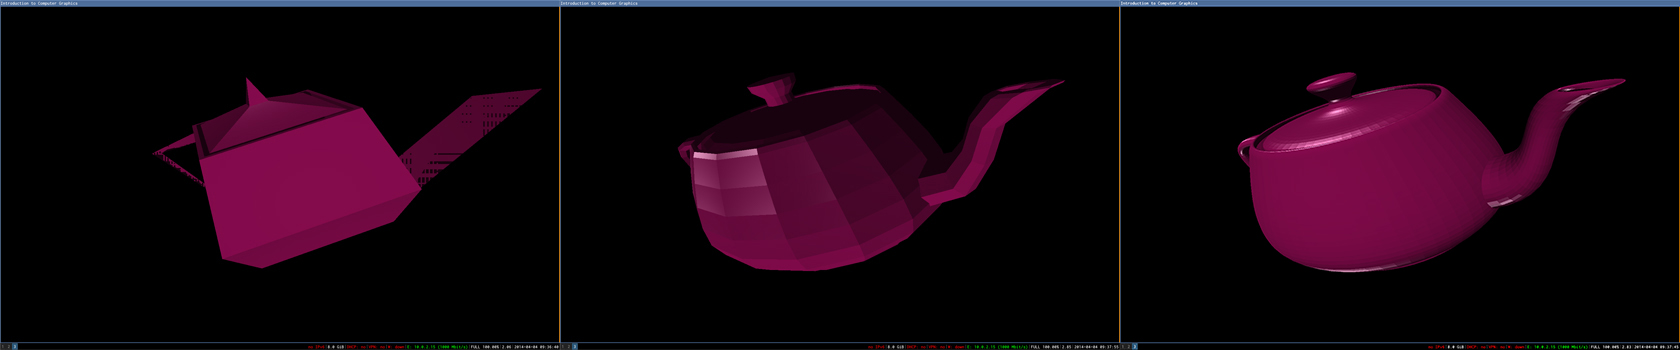
\includegraphics[scale=0.25]{figures/teapot}
    \caption{Renderings of the teapot at different subdivision levels.}
    \label{fig:teapot}
\end{figure}
As can be seen, the algorithm works correctly, as each quad subdivided becomes
four quads. As we increase the number of subdivisions the model becomes
smoother and the light reflected off of it looks increasingly realistic.
\begin{figure}[H]
    \center
    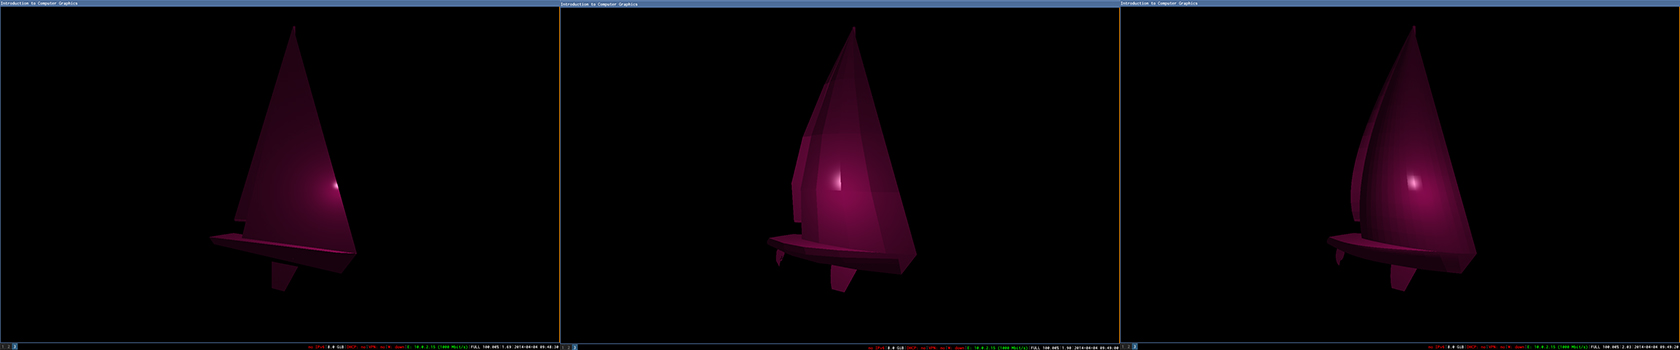
\includegraphics[scale=0.25]{figures/boat}
    \caption{Renderings of the boat at different subdivision levels.}
    \label{fig:boat}
\end{figure}
Do note that I decided not to put any effort into computing vertex normals, as
opposed to face normals, which is what is used. Therefore, the model quads are
still very visible. One could mend this by averaging the face normals who
share a vertex, and aligning them with an index buffer object for the shader
to interpolate these better across the surface. This is outside the scope of
the curriculum, hence the decision of leaving it out.

\subsubsection{Bezier patch surfaces screenshots}
I present a few screenshots of the bezier patch surfaces discussed. Dini's
surface, on the left, uses a two-sided shader which colors backfaces using a
different color. This produces a very pretty surface model that shows both
sides of the model.
\begin{figure}[H]
    \center
    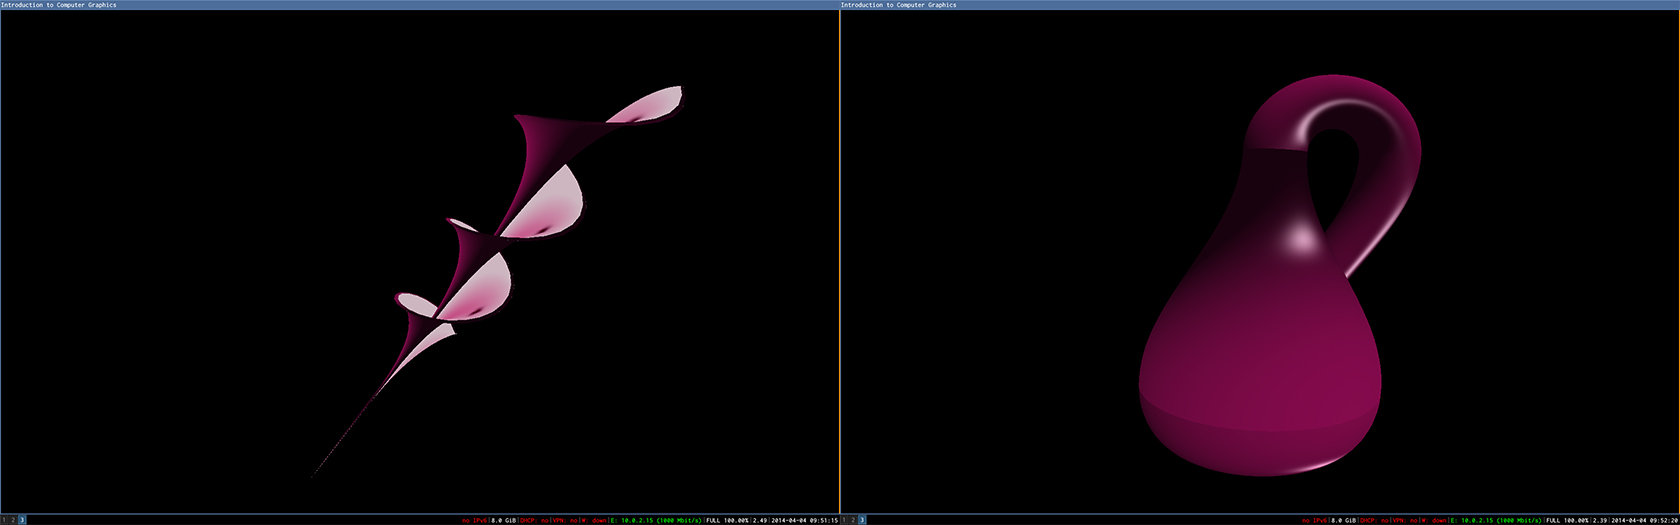
\includegraphics[scale=0.25]{figures/surfaces}
    \caption{Renderings of (left) Dini's surface and (right) the Klein Bottle.}
    \label{fig:surfaces}
\end{figure}
The Klein bottle, on the right, exposes a shader problem. Unfortunately, I did
not get to fix it in time for the assignment delivery, but I believe I know of
where the problem stems from. The shader makes use of an {\it eye} vector,
which is not updated properly, as the camera moves about. Further, another
source of this effect could be that the shader doesn't account properly for
the nature of this model, namely that it has no backside. The way the shader
is constructed, it tries to invert the normals of the surface if a triangle is
facing backward.

\end{document}

